\documentclass{sig-alternate}
\usepackage[USenglish]{babel}
\usepackage[backend=bibtex,style=numeric-comp]{biblatex}
\usepackage{graphicx}
\usepackage{tikz}

\graphicspath{{../figures/}}

\newcommand{\code}[1]{\texttt{#1}}

\author{
\alignauthor{}
Dan Stelljes\\
  \affaddr{Division of Science and Mathematics}\\
  \affaddr{University of Minnesota, Morris}\\
  \affaddr{Morris, Minnesota, USA 56267}\\
  \email{stell124@morris.umn.edu}
}
\conferenceinfo{UMM CSci Senior Seminar Conference, December 2016}{Morris, MN}
\title{Composable Concurrency Models}

\bibliography{references}

\AtEveryBibitem{\clearfield{doi}}
\AtEveryBibitem{\clearfield{note}}

\begin{document}

\maketitle

\begin{abstract}

The need to manage concurrent operations in applications has led to the development of a variety of concurrency models. Modern programming languages generally provide several concurrency models to serve different requirements, and programmers benefit from being able to use them in tandem. We discuss challenges surrounding concurrency control and examine situations in which conflicts between models can occur. Additionally, we describe attempts to implement concurrency models on top of lower-level concurrency abstractions.

\end{abstract}

\keywords{concurrency, parallelism, concurrency abstraction}

\section{Introduction}

Most interactive computer programs depend on concurrency, the ability to perform different tasks at the same time. A web browser, for instance, might at any point be rendering documents in multiple tabs, transferring files, and handling user interaction. On a lower level, the operating system might be running several other applications, juggling background processes, and responding to events~\cite{Swalens2014}. If every long-running process blocked other processes from proceeding, the system would be effectively unusable.

Concurrency models enable programmers to reason about and describe interactions between concurrent processes. The web browser is a good example of several different models: The user interface layer might rely on an event loop, the rendering process might operate in shared memory, and suggestions from browsing history or a search engine might require parallel collection operations to achieve acceptable performance~\cite{Marr2012}.

Given that an application is likely to make use of more than one concurrency model, programmers would prefer that different types of models could be arbitrarily combined. From an engineering standpoint, composable models are also desir\-able---a virtual machine for one or more high-level languages should be able to support a variety of models without resorting to rough low-level approximations. However, different concurrency models are not necessarily composable and unexpected issues may arise when they interact. Recent work has attempted to identify unifying concurrency abstractions that would guarantee composability of different models and also provide underlying virtual machine support~\cite{Marr2009, Marr2012, Swalens2014, Ziv2015}.

\section{Background}

Modern operating systems are expected to run many processes concurrently, and processes themselves are often composed of multiple concurrent threads of execution. A processor can only execute one thread at a time, so multitasking is accomplished by rapidly switching between threads~\cite{Liu1973}. Although concurrent threads may appear to be executed simultaneously, truly parallel execution can only take place across multiple processors.

Concurrency models can abstract over implementation details, allowing programmers to reason in terms of asynchron\-ous tasks and independent components instead of low-level thread management. In addition to making a program more understandable, higher-level models afford a degree of flexibility: Regardless of whether a set of concurrent operations is executed in sequence on one thread, in multiple threads on the same processor, or in parallel on multiple processors, the result will be the same.

\subsection{Concurrency}

For operations to be executed concurrently, they must be able to be executed out of order or in partial order. Lamport, in his foundational work on distributed systems~\cite{Lamport1978}, formalized this by defining a ``happens before'' relation (denoted by ``$\rightarrow$'' and its negation by ``$\nrightarrow$'') on a set of operations: If $A$ and $B$ are operations in the same process and $A$ occurs before $B$, or if $A$ is the sending of a message by one process and $B$ is the receipt of the same message by another process, then $A \rightarrow B$. Two operations $A$ and $B$ are said to be concurrent if $A \nrightarrow B$ and $B \nrightarrow A$.

While the ``happens before'' relation can be used to determine whether operations can be executed concurrently, it does not guarantee the correctness of the results. In a non-concurrent (entirely sequential) program, it would be sufficient to show that the program is correct after the execution of each operation and therefore correct upon termination. In other words, the program could be proved to be correct by proving that its history (that is, the sequence in which its operations are performed) yields a correct result. Consistency models guarantee the correctness of a program by defining a set of all allowed histories, or histories that lead to a correct result~\cite{Ziv2015}. If an execution of a program follows an allowed history, the execution is consistent. If not, the execution is inconsistent. If every possible execution of the program follows an allowed history, the program conforms to the consistency model.

\begin{figure}[h]
  \centering
  \resizebox{\linewidth}{!}{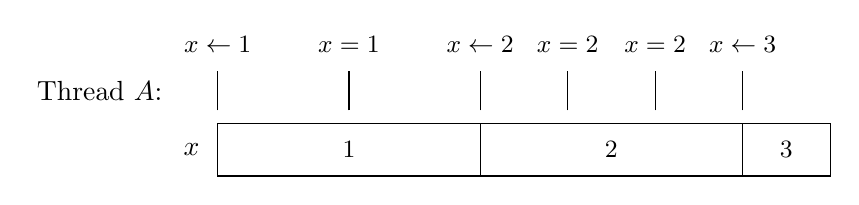
\begin{tikzpicture}
  \node at (-6.5,0.75) { Thread $A$: };
  \node at (-5.333,0) { $x$ };

  \draw (-5,-0.333) rectangle (-1.667,0.333) node [midway] { \small $1$ };
  \draw (-1.667,-0.333) rectangle (1.667,0.333) node [midway] { \small $2$ };
  \draw (1.667,-0.333) rectangle (2.778,0.333) node [midway] { \small $3$ };

  \draw (-5,0.5) -- (-5,1) node [above=3pt] { \small $x \leftarrow 1$ };
  \draw (-3.333,0.5) -- (-3.333,1) node [above=3pt] { \small $x = 1$ };

  \draw (-1.667,0.5) -- (-1.667,1) node [above=3pt] { \small $x \leftarrow 2$ };
  \draw (-0.555,0.5) -- (-0.555,1) node [above=3pt] { \small $x = 2$ };
  \draw (0.555,0.5) -- (0.555,1) node [above=3pt] { \small $x = 2$ };

  \draw (1.667,0.5) -- (1.667,1) node [above=3pt] { \small $x \leftarrow 3$ };
\end{tikzpicture}
}
  \caption{A single thread writes to and reads from a variable.}
\label{figure:single}
\end{figure}

Figure~\ref{figure:single} illustrates a simple program in which a single thread reads and writes numbers from a variable $x$. The value of $x$ over time is represented by a segmented bar. Write operations are denoted by an arrow pointing toward the bar and read operations by an arrow pointing away. The program satisfies an intuitive model of how variables should behave---each time $x$ is read, the value is equal to the value of the most recent write.

\begin{figure}[h]
  \centering
  \resizebox{\linewidth}{!}{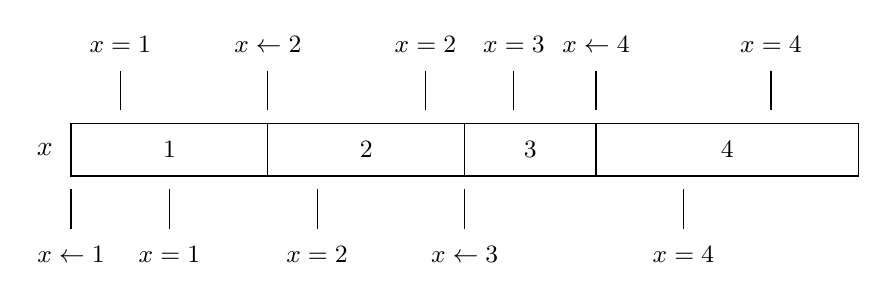
\begin{tikzpicture}
  \node at (-5.333,0) { $x$ };

  \draw (-5,-0.333) rectangle (-2.5,0.333) node [midway] { \small $1$ };
  \draw (-2.5,-0.333) rectangle (0,0.333) node [midway] { \small $2$ };
  \draw (0,-0.333) rectangle (1.667,0.333) node [midway] { \small $3$ };
  \draw (1.667,-0.333) rectangle (5,0.333) node [midway] { \small $4$ };

  \draw (-5,-0.5) -- (-5,-1) node [below=3pt] { \small $x \leftarrow 1$ };
  \draw (-4.375,0.5) -- (-4.375,1) node [above=3pt] { \small $x = 1$ };
  \draw (-3.75,-0.5) -- (-3.75,-1) node [below=3pt] { \small $x = 1$ };

  \draw (-2.5,0.5) -- (-2.5,1) node [above=3pt] { \small $x \leftarrow 2$ };
  \draw (-1.875,-0.5) -- (-1.875,-1) node [below=3pt] { \small $x = 2$ };
  \draw (-0.5,0.5) -- (-0.5,1) node [above=3pt] { \small $x = 2$ };

  \draw (0,-0.5) -- (0,-1) node [below=3pt] { \small $x \leftarrow 3$ };
  \draw (0.625,0.5) -- (0.625,1) node [above=3pt] { \small $x = 3$ };

  \draw (1.667,0.5) -- (1.667,1) node [above=3pt] { \small $x \leftarrow 4$ };
  \draw (2.778,-0.5) -- (2.778,-1) node [below=3pt] { \small $x = 4$ };
  \draw (3.889,0.5) -- (3.889,1) node [above=3pt] { \small $x = 4$ };
\end{tikzpicture}
}
  \caption{Two threads concurrently write to and read from a variable.}
\label{figure:multiple}
\end{figure}

In a concurrent program, the history of operations may not be the same for every execution. As a result, assumptions about correctness that are true for a sequential program may be violated in a concurrent program. This is illustrated in Figure~\ref{figure:multiple}, in which two threads concurrently write from and read to a variable $x$ concurrently. Because the operations of the threads are interleaved, a read operation on $x$ may not yield a value that matches the value of that thread's most recent write. The value may even be inconsistent between consecutive reads. If a single thread were to incorrectly assume that it had exclusive control of $x$, this behavior would appear incorrect and could lead to race conditions, errors that arise due to unintentional dependency on execution order.

\subsection{Linearizability}

The examples above assume that all operations complete instantaneously. In real systems, though, operations take time. Even writing to a location in cache memory, an operation measured in nanoseconds, is not truly instantaneous. That an operation may be completed at a time significantly later than the time at which it was invoked introduces uncertainty into a history of operations---the sequence of execution may be influenced by the time it takes for messages to travel.

\begin{figure}[h]
  \centering
  \resizebox{0.63\linewidth}{!}{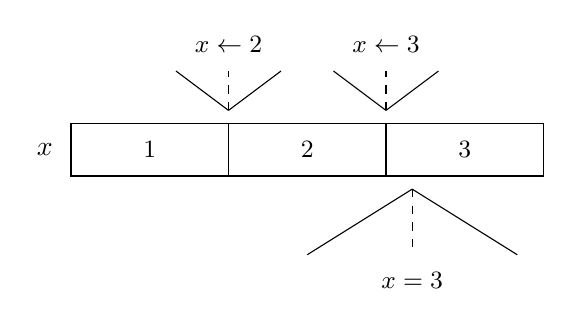
\begin{tikzpicture}
  \node at (-3.333,0) { $x$ };

  \draw (-3,-0.333) rectangle (-1,0.333) node [midway] { \small $1$ };
  \draw (-1,-0.333) rectangle (1,0.333) node [midway] { \small $2$ };
  \draw (1,-0.333) rectangle (3,0.333) node [midway] { \small $3$ };

  \draw (-1.667,1) -- (-1,0.5) (-1,0.5) -- (-0.333,1);
  \draw [dashed] (-1,0.5) -- (-1,1) node [above=3pt] { \small $x \leftarrow 2$ };

  \draw (0.333,1) -- (1,0.5) (1,0.5) -- (1.667,1);
  \draw [dashed] (1,0.5) -- (1,1) node [above=3pt] { \small $x \leftarrow 3$ };

  \draw (0,-1.333) -- (1.333,-0.5) (1.333,-0.5) -- (2.667,-1.333);
  \draw [dashed] (1.333,-0.5) -- (1.333,-1.333) node [below=3pt] { \small $x = 3$ };
\end{tikzpicture}
}
  \caption{Two threads concurrently (and noninstantaneously) write to and read from a variable.}
\label{figure:time}
\end{figure}

Consider a third example (Figure~\ref{figure:time}) in which two threads interact with a variable $x$ noninstantanously. Invocation is denoted by the leftmost point of an event and completion by the rightmost point. The dotted line indicates the instant at which the operation takes effect. The lower thread invokes a read while the value of $x$ is set to $1$. The upper thread invokes and completes a write between the time that the read is invoked and the value is actually read. The read operation then returns $2$ even though $x$ was equal to $1$ at the time it was invoked.

While travel time may introduce ambiguity, there are still some restrictions on possible sequences of events. Specifically, an operation cannot take effect before its invocation, nor can it take effect after its completion. Therefore, assuming that all threads share some single global state and that operations on that state take place atomically, each operation will appear to take effect atomically at some point after it is invoked and before it is completed.

\begin{figure}[h]
  \centering
  \resizebox{0.63\linewidth}{!}{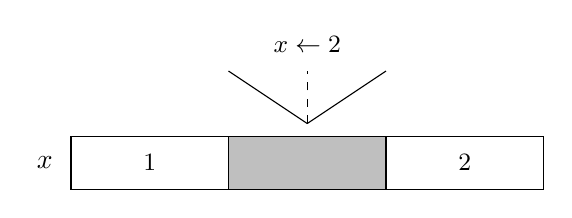
\begin{tikzpicture}
  \node at (-3.333,0) { $x$ };

  \draw (-3,-0.333) rectangle (-1,0.333) node [midway] { \small $1$ };
  \draw [fill=lightgray] (-1,-0.333) rectangle (1,0.333);
  \draw (1,-0.333) rectangle (3,0.333) node [midway] { \small $2$ };

  \draw (-1,1.167) -- (0,0.5) (0,0.5) -- (1,1.167);
  \draw [dashed] (0,0.5) -- (0,1.167) node [above=3pt] { \small $x \leftarrow 2$ };
\end{tikzpicture}
}
  \caption{A single thread performs an atomic write operation on a variable.}
\label{figure:linearizability}
\end{figure}

This consistency model is referred to as linearizability (also referred to as atomicity or indivisibility), and it guarantees that the completion of an operation on a single object will appear to the rest of the system to be instantaneous~\cite{Herlihy1990}. In other words, even though linearizable operations are executed concurrently and take time, they appear to happen in a simple linear order. Figure~\ref{figure:linearizability} demonstrates an atomic write on a variable $x$: Although the operation takes time, the entire operation (denoted by the shaded area) can be collapsed into one apparently instantaneous event.

A useful consequence of linearizability is that the results of an operation must be visible as soon as the operation is complete. This can prevent issues such as stale reads (in which a read operation returns a value different from the most recently written value) and non-monotonic reads (in which a later read operation returns an older value than an earlier read operation). Linearizability is also a composable guarantee~\cite{Herlihy1990}---an operation made up of smaller linearizable operations is itself linearizable.

\subsection{Serializability}

A history of operations is said to be serializable if it is equivalent to a serial (i.e., non-interleaved) ordering of its operations~\cite{Herlihy1990}. Serializability is like linearizability in that it demands some linear order of execution. However, serializability describes multiple operations over multiple objects instead of single operations on single objects, and it does not impose any wall-clock time constraints on the history. This means that operations may occur in any order as long as some serial history exists.

\begin{figure}[h]
  \centering
  \resizebox{0.63\linewidth}{!}{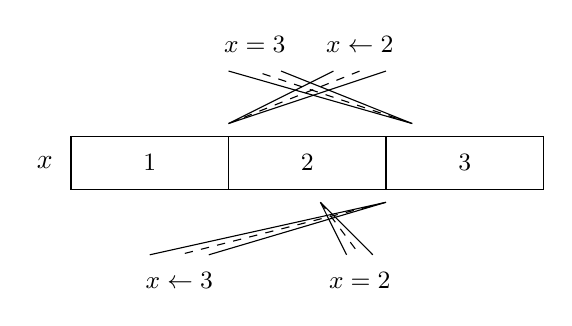
\begin{tikzpicture}
  \node at (-3.333,0) { $x$ };

  \draw (-3,-0.333) rectangle (-1,0.333) node [midway] { \small $1$ };
  \draw (-1,-0.333) rectangle (1,0.333) node [midway] { \small $2$ };
  \draw (1,-0.333) rectangle (3,0.333) node [midway] { \small $3$ };

  \draw (0.333,1.167) -- (-1,0.5) (-1,0.5) -- (1,1.167);
  \draw [dashed] (-1,0.5) -- (0.667,1.167) node [above=3pt] { \small $x \leftarrow 2$ };

  \draw (0.5,-1.167) -- (0.167,-0.5) (0.167,-0.5) -- (0.833,-1.167);
  \draw [dashed] (0.167,-0.5) -- (0.667,-1.167) node [below=3pt] { \small $x = 2$ };

  \draw (-2,-1.167) -- (1,-0.5) (1,-0.5) -- (-1.25,-1.167);
  \draw [dashed] (1,-0.5) -- (-1.625, -1.167) node [below=3pt] { \small $x \leftarrow 3$ };

  \draw (-1,1.167) -- (1.333,0.5) (1.333,0.5) -- (-0.333,1.167);
  \draw [dashed] (1.333,0.5) -- (-0.667,1.167) node [above=3pt] { \small $x = 3$ };
\end{tikzpicture}
}
  \caption{Two threads perform a set of serializable read and write operations on a variable.}
\label{figure:serializability}
\end{figure}

Figure~\ref{figure:serializability} illustrates a set of serializable read and write operations. Even though the exeuctions of each operation occur out of order and even intersect, the events themselves can be arranged serially: $x \leftarrow 1$, $x = 1$, $x \leftarrow 2$, $x = 2$.

Serializability alone is a fairly weak consistency model. Because it does not place bounds on time or order, events may happen out of sequence, and, unlike linearizability, serializability is not a composable guarantee. Serializability is useful, though, as a guarantee of isolation~\cite{Haerder1983}: While a serializable set of operations is being executed, it appears to be the only set of operations being executed. For histories to be serializable, then, they must not overlap and cannot interfere with each other.

Together, linearizability and serializability guarantee strict serializability, in which a history is equivalent to a serial execution order and that serial order corresponds to the execution order in real time. Given that, linearizability can actually be described as strict serializability restricted to single operations on single objects~\cite{Herlihy1990}.

\section{Common concurrency models}

Modern programming languages generally provide several different concurrency models, each with their own terminology and specific implementation details. It would be impractical to discuss them all, but the most commonly used models can be adequately described by generalization~\cite{Swalens2014}.

\subsection{Atomic variables}

Atomic variables are used to share independent objects that do not demand coordinated updates but need to be shared by multiple threads~\cite{Swalens2014}. Atomic variables can only be read and mutated by operations that are guaranteed to be linearizable. For example, the atomic operation \code{compare-and-swap} compares the current value of a variable to a given value and only performs a write if the values match~\cite{Swalens2014}. \code{compare-and-swap} ensures that a new value cannot be written based on outdated information. Suppose that a thread $A$ reads a variable $x$ and begins computing a new value. At the same time, another thread $B$ modifies $x$. When $A$ tries to set the value of $x$ via \code{compare-and-swap}, the write will fail. As a result, all writes on $x$ are guaranteed to be linearizable.

Atomic operations are often implemented in hardware and guarantee linearizability at the lowest level possible. \code{fetch-and-add}, another atomic operation, is a common processor instruction that executes multiple hardware-level operations: The value old value is copied from a location in memory into a temporary register, addition is performed on the value in the temorary register, and the new value is stored at the original location.

Atomic variables often serve as the basis for higher-level concurrency control mechanisms such as semaphores and locks, which in turn support the implementation of concurrent data structures. A counting semaphore is an atomic variable that serves as a record of how many units of a shared resource are available. By taking advantage of atomic operations, the semaphore can be safely updated and will reliably determine whether a shared resource can be used. A single thread can then test if a resource is available and acquire it before proceeding, thereby preventing race conditions~\cite{Swalens2014}. A lock (also referred to as a mutex) guarantees mutual exclusion, which requires that two threads cannot operate on a shared object at the same time. Locks are commonly implemented by a binary semaphore (that is, a semaphore that simply indicates whether a single resource is available).

Many higher-level languages (such as Clojure~\cite{Swalens2014}) provide atomic references that can be read by an atomic dereferencing operation and written by an atomic swap operation. Such operations may provide convenience features such as automatic retries.

\subsection{Software transactional memory}

Software transactional memory (STM) presents an alternative to semaphores and locks by allowing multiple concurrent operations to write to a shared location in memory. STM is an example of optimistic concurrency control: Each thread executes a series of read and write operations (called a transaction) on the shared memory without considering the activity of other threads. On its face, this approach seems disaster-prone---multiple threads writing to the same memory location could easily lead to corrupted data. STM solves this problem by recording all operations in a log. After the entire transaction is completed, the transaction manager verifies that other threads have not also made changes to the shared memory. If there are conflicting changes, the transaction is aborted and retried until it eventually succeeds~\cite{Shavit1995}.

Conceptually, STM simplifies concurrency because it allows a transaction to be thought of as a single strictly serializable operation. A thread cannot observe changes made to other threads while a transaction is in progress, nor can other threads observe modifications by that thread until the transaction is completed. Only when a transaction completes successfully will changes will become visible to other threads. Practically, STM is useful in any situation in which a shared object needs to be accessed and modified by multiple threads~\cite{Swalens2014}.

STM also offers significant advantages over lock-based programming in terms of composability. Given that executing two operations within a transaction yields a larger atomic operation, Harris et al.\ describe a STM that allows any combination of atomic operations to be composed into a larger atomic operation~\cite{Harris2005}.

However, the requirement that transactions must be able to be aborted and retried places constraints on the set of allowed operations. Specifically, a transaction cannot execute any operation that cannot be undone or retried, such as writing to disk or performing a network request. STM can also result in a decrease in performance caused by the overhead of maintaining the log and aborting and retrying transactions.

\subsection{Communicating threads}

Other concurrently models avoid the use of shared memory (and the problems that arise from doing so) by restricting threads to private memory. Threads communicate strictly by message passing, which avoids race conditions. A variety of different communicating thread models exist and have long been a solution to describing concurrent operations. Practical use cases for communicating threads include communication with external systems or running an event loop~\cite{Swalens2014}.

Communicating sequential processes (CSP), one of the oldest communicating thread models, describes systems in terms of independent processes that communicate through predefined channels~\cite{Hoare1978}. CSP is notable in that messages are passed synchronously; that is, a sending process will block until a complementary operation is executed on the receiving process~\cite{Swalens2014}.

Other models, most notably the actor model, rely on asynchronous message passing to specific entities~\cite{Agha1986}. Actors can only communicate via asynchronous message passing. Upon receiving a message, an actor can choose to send messages to other actors, create new actors, and determine the behavior used for the next received message.

Shared state can also be represented by communicating threads. The agent model, for instance, works similarly to atomic references. A state wrapped by an agent can be modified by a message that sends an updated state. The value can be accessed by a dereferencing operation that reads the current value from the agent~\cite{Swalens2014}.

\subsection{Proxies}

Proxies are a general term used to describe placeholders for values that are the result of some concurrently executed operation. Unlike communicating thread models, which rely on message passing between dedicated threads, a proxy executes some function in a new thread and delivers the result upon completion~\cite{Swalens2014}.

Futures and promises are two of the most common proxy models, though the terms are frequently used interchangeably (along with ``delayed,'' ``deferred,'' and ``eventual''). Generally, futures are resolved to the result of the completed operation. The result is then accessed implicitly; any use of the future will return its value. Promises, on the other hand, are created as independent objects and require the result to be accessed explicitly.

In practice, proxies are used to execute long-running operations such as rendering or network requests~\cite{Swalens2014} without blocking other operations. Promise objects, which can be easily passed and composed, generally offer more flexibility than constructs such as asynchronous callbacks~\cite{Kambona2013}.

\section{Composability challenges}

While concurrency models guarantee their own correctness, issues may arise when different models are used together. For example, an implementation of a STM that guarantees linearizability assumes that all shared resources are managed by the STM~\cite{Shavit1995}. However, if a thread communicates with other threads (in CSP, for instance), that assumption could lead to unexpected interleaving of operations~\cite{Swalens2014}.

Swalens et al.~\cite{Swalens2014}, in a through study of concurrency models provided by Clojure, examined issues that arise when different models are combined. Two models are said to be composable if combining them does not introduce correctness issues.

\subsection{Correctness criteria}

In the study, safety and liveness were used as the two criteria for evaluating the correctness of a combination of models. Together, the two have historically been used to prove the correctness of distributed systems~\cite{Lamport1977}.

Informally, safety guarantees that ``nothing bad will happen.'' In other words, given a correct input, a program will not produce an incorrect result~\cite{Swalens2014}. This property is also referred to as partial correctness. Safety is generally achieved in the management of shared resources. STM, for instance, only allows shared memory to be accessed through transactions; communicating threads only allow data to be shared through message passing.

Liveness guarantees that ``something good will eventaully happen,'' or that a program will eventually terminate if its input is correct. Taken together, safety and liveness are referred to as total correctness---given a correct input, a program will terminate with the correct output~\cite{Swalens2014}. Deadlocks and livelocks are the primary obstacle to liveness and can arise when models are combined.

\subsection{Possible conflicts}

To discover the types of conflicts that might arise when combining different models, the study examined all pairwise combinations of Clojure's models. This process uncovered the following types of conflicts:

\begin{itemize}
  \item A model reexecutes code containing another concurrency model that performs an irrevocable action. (A STM transaction contains a proxy that performs a network request.)

  \item A model reexecutes code that causes the reexecution to continually happen. (An STM transaction that consistently conflicts with another may cause a livelock, though Swalens et al.~note that Clojure dynamically prevents this type of conflict.)

  \item A model that supports blocking operations is used within a model that does not expect blocking operations. (A deadlock might be caused when a read operation occurs within mutually recursive futures.)

  \item A model does not guarantee safety or liveness by design, making composability impossible. (A model that does not guarantee safety would violate the safety guarantee of an outer model unless such a conflict was explicitly prevented.)
\end{itemize}

\section{Proposed abstractions}

%\subsection{Asynchronous events}

% Ziarek et al.~\cite{Ziarek2011} introduce asynchronous events as a possible abstraction. Their examples are heavily tied to Concurrent ML and might be difficult to integrate.

\subsection{Ownership-based meta-object protocol}

Marr and D'Hondt~\cite{Marr2012} surveyed a variety of concurrent and parallel programming concepts to identify a unifying concurrency abstraction that could be implemented at the virtual machine level.\footnote{A 2009 survey by Marr, Haupt, and D'Hondt~\cite{Marr2009} found that virtual machines at the time did not provide intrinsic support for more than one specific model.} A unifying abstraction would enable each concurrency model in a high-level language to be represented in machine code without sacrificing performance or semantics. To identify concepts relevant for a multi-language virtual machine, Marr and D'Hondt selected four questions:

\begin{enumerate}
  \item Can the concept be reasonably implemented as a library? (A library implementation may suffer from loss of performance or semantics to an extent that the concept would warrant virtual machine inclusion.)

  \item Does the concept require runtime support to guarantee its semantics? (Semantic guarantees may be enforced by a compiler but not the virtual machine. For instance, immutable objects in one language may not be immutable in machine code, and therefore may be mutated by another language.)

  \item Would runtime support benefit performance? (Deeper knowledge of the concept may enable the virtual machine to better optimize. Some concepts, though, may require knowledge of the underlying hardware to realize any performance improvements; such concepts would not necessarily benefit from runtime support.)

  \item Is the concept already supported by a common virtual machine like the Java Virtual Machine (JVM) or the Common Language Runtime (CLR)?
\end{enumerate}

From those questions, 26 concepts were identified that would benefit from better low-level support. Of those, 18 suffered from loss of semantic guarantees when compiled to machine code. With that in mind, Marr and D'Hondt derived the following requirements for a unifying abstraction:

\begin{itemize}
  \item Managed mutation: Concurrency models impose restrictions on how state can be modified; therefore, mutation must be able to be flexibly managed.

  \item Managed execution: Similarly, invocation of operations on objects is usually restricted and must be able to be flexibly managed.

  \item Ownership: Some owning entity usually regulates mutation and execution, so ownership should be supported in a way that allows for adaptable mutation and execution rules.

  \item Leveled reflection: Reflection allows a program to examine its own structure and behavior at runtime. To guarantee safety, there needs to be a distinction between language-level reflection (restricted reflection operations supported by the high-level language) and meta-level reflection (unrestricted reflection operations on the low-level abstraction).

  \item Enforceability: All defined restrictions should be enforceable on different concurrency models. Additionally, the semantics of the language in which a model is defined must be enforced regardless of where the model is used.
\end{itemize}

\begin{figure}[h]
  \centering
  \includegraphics[width=224pt]{obmop}
  \caption{Marr and D'Hondt's object-based meta-object protocol~\cite{Marr2012}.}
\label{figure:obmop}
\end{figure}

Given those requirements, Marr and D'Hondt defined an ownership-based meta-object protocol (MOP) that could describe a low-level abstraction, illustrated in Figure~\ref{figure:obmop}. The owner of an object, referred to as the domain, manages operations on all of the objects that it owns (namely, reading and writing of object fields and invocation of methods on objects). This satisfies the ownership requirement. Read and write operations are directed to the \code{readField} and \code{writeField} operations on the domain, satisfying the managed mutation requirement. Similarly, all method invocations are directed to the \code{exec}, satisfying the managed execution requirement. Threads are executed in a domain and specify whether execution occurs at the language level (with restricted reflection) or the meta level (with unrestricted reflection), satisfying the leveled reflection requirement. Globally shared resources are handled by the domain (specifically, the \code{readGlobal} and \code{writeGlobal} methods) if they might break semantics. Additionally, the \code{primitive*} operations allow callers to override the semantics of virtual machine primitives, completing the enforcability requirement.

To demonstrate the suitability of the MOP as a low-level abstraction, Marr and D'Hondt implemented several concurrency models. The MOP was able to support LRSTM (a STM for the Smalltalk language), Clojure's agents (which rely on communicating threads), active objects (a variation on proxies), and several other models. While the MOP was able to successfully enforce the semantics of each model, the resulting performance cost suggested that the MOP must be implemented at the virtual machine level to sufficiently reduce the abstraction overhead. Marr and D'Hondt also note that regarding the owner of an object as the only entity able to restrict interaction is somewhat limiting. For instance, the behavior of the system when different semantics interact needs to be explicitly specified.

\section{Conclusion}

In more words: There's a lot of work on the correctness of concurrent operations. With some care, concurrency models can be composed. There's some work on deeper abstractions, but it's definitely ongoing and more is likely to follow soon.

\section*{Acknowledgments}

Thanks to Elena Machkasova and K.~K. Lamberty for their patience and feedback.

\printbibliography{}

\end{document}
